%%%%%%%%%%
%
% DIRECTIONS
% Students count off 1, 2, 3, ..., 7
% Then each does that number (or takes a guess)
% Then explains their answer to their neighbor
% Volunteers write their answers on a copy
%   under a document camera.
%
%%%%%%%%%%

\RequirePackage{luatex85}
\documentclass[10pt, addpoints]{exam}
\usepackage{tikz, pgfplots, amsmath, mathtools, multicol}
%\pgfplotsset{compat=1.15}
\usepackage[letterpaper, margin=0.5in, column sep=1in]{geometry}
\setlength\parindent{0mm}

% \usepackage{expl3}
% \ExplSyntaxOn
% \cs_new_eq:NN \Repeat \prg_replicate:nn
% \ExplSyntaxOff

\newcommand\content[5]{\question $\left\{\begin{aligned}
	\phantom{\lim_{x\to \mathbf{#1}^+}} f(#1) &= \ifprintanswers #2 \fi
	\\[-0.5ex] \lim_{x\to \mathbf{#1}^-}f(x) &= \ifprintanswers #3 \fi
	\\[-0.5ex] \lim_{x\to \mathbf{#1}^+}f(x) &= \ifprintanswers #4 \fi
	\\[-0.5ex] \lim_{x\to \mathbf{#1}\phantom{^+}}f(x) &= \ifprintanswers #5 \fi
	\end{aligned}\right.$}

\newcommand{\gaacard}[4]{
\question
$\begin{matrix}
\begin{tikzpicture}
\begin{axis}[
	every axis/.append style={font=\tiny}, 
	xmin=-3.1, xmax=3.1,
	ymin=-2.4, ymax=2.4,
	samples=99, 
	major tick length={0},
	line width=1pt,
	axis lines=center, height=1.6in, width=2in, grid=major,
	restrict y to domain=-2.4:2.4, 
%	title={\normalsize{\unboldmath$\displaystyle f(x) = #1$}},
	extra y tick style={y tick label style={right}},
	#3,
%	samples=59 %COMMENT OUT
	]
	\addplot [black, smooth, thick, domain=-3:3] {#2};
	#4
\end{axis}
\end{tikzpicture}
\end{matrix}$

\vspace{-3mm}
\fullwidth{$\begin{aligned}
	\phantom{\lim_{x\to \mathbf0^+}} f(x) &= \smash{#1}
	\\[-0.9ex] \phantom{\lim_{x\to \mathbf0^+}} f(0) &=
	\\[-0.9ex] \lim_{x\to \mathbf0^-}f(x) &=
	\\[-0.9ex] \lim_{x\to \mathbf0^+}f(x) &=
	\\[-0.9ex] \lim_{x\to \mathbf0\phantom{^+}}f(x) &=
	\\[-0.9ex] \lim_{x\to \mathrlap{-\infty}\phantom{\mathbf0{^+}}}f(x) &=
	\\[-0.9ex] \lim_{x\to \mathrlap{+\infty}\phantom{\mathbf0{^+}}}f(x) &=
	\end{aligned}$}
}

\newcommand\gacard[3]{\gaacard{#1}{#2}{#3}{}}
\newcommand\gcard[2]{\gacard{#1}{#2}{grid=none, ticks=none}}
\newcommand\opencircle[1]{\draw[color=black,fill=white,thick] (axis cs:{#1}) circle [radius=2pt];}

\thispagestyle{empty}
\pagestyle{empty}
\begin{document}


% set amount to shrink in y direction first diagram
\def\yscaleone{3}
\newcommand\diagram{
\fullwidth{
\begin{center}
\begin{tikzpicture}
	[very thick, yscale=1/\yscaleone]
	% grid
	\draw[gray, semithick] (-1,0) grid (14.25,20.5);
	% x- and y-axes
	\draw[<->, semithick] (-1,21) -- 
		node[pos=0.03, right] {$y$} (-1,0) --  
		node[pos=0.99, above] {$x$} (14.5,0);
	% labels on y-axis
	\foreach \y in {0,10,...,200}
	\draw (-1,\y/10) node[left] {\y};
	% labels on x-axis
	\foreach \x in {1,...,12}
	\draw (\x,0) node[below] {\x};
	% vertical asymptotes
	\foreach \x in {8,...,12}
	\draw[dashed, semithick] (\x,0) -- (\x,20.5);
	% horizontal asymptotes
	\foreach \y in {9,6}
	\draw[dashed, semithick] (-1,\y) -- (14.25,\y);
	% plot five curves on left half
	\draw[smooth] plot coordinates{(-1,8.9) (0.2,8.6) (1,7) (2,2) (3.15,1.15) (4,5)};
	\draw (4,8) -- (5,7);
	\draw (5,16) to [bend right=10] (6,10);
	\draw (6,14) -- (7,13);
	\draw (7,17) to [bend left=10]  (8,11);
	% plot five asymptotic curves on right half
	\draw[smooth] plot coordinates {(8.1,20.5) (8.2,15) (8.8,15) (8.9,20.5)};
	\draw[smooth] plot coordinates {(9.1,20.5) (9.2,12) (9.8,8) (9.9,0)};
	\draw[smooth] plot coordinates {(10.1,20.5) (10.2,13) (10.8,13) (10.9,20.5)};
	\draw[smooth] plot coordinates {(11.1,0) (11.2,10.5) (11.8,10.5) (11.9,0)};
	\draw[smooth] plot coordinates {(12.1,0) (12.4,5) (14.25,5.85)};
	% open circles
	\foreach \x/\y in {2/2, 3/1, 4/5, 4/8, 5/7, 5/16, 6/10, 7/17, 8/11}
	\draw[black, fill=white, yscale=\yscaleone] (\x,\y/\yscaleone) circle (3pt);
	% closed circles
	\foreach \x/\y in {3/4, 5/19, 6/14, 7/13, 8/3, 11/15, 12/18}
	\draw[black, fill=black, yscale=\yscaleone] (\x,\y/\yscaleone) circle (2.5pt);
	% f(x) label
	\draw (1.5,15) node[fill,white] {\color{black} \huge$f(x)$};
	\end{tikzpicture}
	\end{center}
	}
	
	\vspace{-1em}
	}

\diagram
\begin{questions}
\section{Finding Limits Graphically}
\begin{multicols}{3}
	\content1{}{}{}{}
	\content2{}{}{}{}
	\content3{10}{}{}{}
	\content4{}{}{}{}
	\content5{}{}{}{}
	\content6{}{}{}{}
	\content7{}{}{}{}
	\end{multicols}

\renewcommand\content[5]{\question $\left\{\begin{aligned}
	\phantom{\lim_{x\to \mathbf{#1}^+}} g(#1) &= #2
	\\[-0.5ex] \lim_{x\to \mathbf{#1}^-}g(x) &= #3
	\\[-0.5ex] \lim_{x\to \mathbf{#1}^+}g(x) &= #4
	\\[-0.5ex] \lim_{x\to \mathbf{#1}\phantom{^+}}g(x) &= #5
	\end{aligned}\right.$}

\section{Infinite Limits and Limits at Infinity}
\begin{multicols}{3}
	\content8{}{}{}{}
	\content9{}{}{}{}
	\content{10}{}{}{}{}
	\content{11}{}{}{}{}
	\content{12}{}{}{}{}
	\bigskip
	\question $\lim\limits_{x\to \mathbf{-\infty}}g(x) =$
	\question $\lim\limits_{x\to \mathbf{+\infty}}g(x) =$
	\end{multicols}

\clearpage
\setlength\columnsep{8mm}
\raggedcolumns
\begin{multicols}4
	\gcard{1/x}{1/x}
	\gcard{1/x^2}{1/x/x}
	\gcard{|x|}{abs(x)}
	\gaacard{\sqrt[3]x}{0}{grid=none, ticks=none}{\addplot[black, smooth, thick, domain=-3:3] (x^3,x);}
	\end{multicols}

\vfill
\begin{multicols}4
	\gcard{x^3}{x^3}
	\gacard{e^x}{e^x}{ytick={1}, xtick={0}}
	\gacard{\ln(x)}{ln(x)}{ytick={0}, xtick={1}}
	\gaacard{\frac{\left| x \right|}x}{floor(x/10)*2+1}{ytick={1},extra y ticks={-1},xtick={0},samples={501}}{\opencircle{0,1} \opencircle{0,-1}}
	\end{multicols}

\vfill
\begin{multicols}4
	\gacard{\cos(x)}{cos(deg(x)*2)}{ytick={-1,1},xtick={0}}
%	\gaacard{\frac{\sin(x)}x}{sin(deg(x*3))/(x*3)}{ytick={-1,1},xtick={0}}{\opencircle{0,1}}
	\gaacard{\frac{\sin(x)}x}{cos(deg(x*6))*exp(-abs(x/1.25))}{ytick={-1,1},xtick={0}}{\opencircle{0,1}}
	\gacard{\sin(1/x)}{sin(deg(1/x*1.5))}{ytick={-1,1},xtick={0},samples={720}}
	\gacard{x\sin(1/x)}{x/3*sin(deg(1/x*3))}{ytick={-1,1},xtick={0},samples={720}}
	\end{multicols}

\newpage
\diagram
\section{Identify Continuity/Discontinuity at a Point} %(removable, jump, infinite)
\question We say $f(x)$
	is  \fillin[\textbf{continuous at $x=a$}][2in] 
	if $\lim\limits_{x\to a}f(x)$ exists and equals $f(a)$.
\question We say $f(x)$
	has a \fillin[\textbf{removable discontinuity at $x=a$}][2in] at $x=a$ 
	if $\lim\limits_{x\to a}f(x)$ exists and does \emph{not} equal $f(a)$.
\question We say $f(x)$
	has a \fillin[\textbf{jump discontinuity at $x=a$}][2in]
	if $\lim\limits_{x\to a^+}f(x)$ and $\lim\limits_{x\to a^-}f(x)$ exist and are \emph{un}equal. 
\question We say $f(x)$
	has an \fillin[\textbf{infinite discontinuity at $x=a$}][2in]
	if either $\lim\limits_{x\to a^+}f(x)$ or $\lim\limits_{x\to a^-}f(x)$
	equals either $\infty$ or $-\infty$.

\question The function $f(x)$ is \textbf{continuous at \boldmath $x$ =} \fillin[][3in].
\question The function $f(x)$ is has a \textbf{removable discontinuity at \boldmath $x$ =} \fillin[][3in].
\question The function $f(x)$ is has a \textbf{jump discontinuity at \boldmath $x$ =} \fillin[][3in].
\question The function $f(x)$ is has an \textbf{infinite discontinuity at \boldmath $x$ =} \fillin[][3in].

\section{Identify Left and Right Continuity at a Point}
\question We say $f(x)$ is \fillin[left continuous at $x=a$][3in]
	if $\lim_{x\to a^-}f(x)$ exists and equals $f(a)$.
\question We say $f(x)$ is \fillin[right continuous at $x=a$][3in]
	if $\lim_{x\to a^+}f(x)$ exists and equals $f(a)$.

\question The function $f(x)$ is \textbf{left continuous at \boldmath $x$ =} \fillin[][3in].
\question The function $f(x)$ is \textbf{right continuous at \boldmath $x$ =} \fillin[][3in].

\section{Continuity on an Interval}
We say $f(x)$ is \textbf{continuous on \boldmath $(a,b)$}
	if $f(x)$ is continuous at $x=c$ for all $c$ in $(a,b)$.
\question We say $f(x)$ is \textbf{continuous on \boldmath $[a,b]$}
	if $f(x)$ is continuous at $x=c$ for all $c$ in $(a,b)$, \\[3ex]
	and \fillin[right continuous at $x=a$][3in]
	and \fillin[left continuous at $x=a$][3in].
\question We say $f(x)$ is \textbf{continuous everywhere}
	if $f(x)$ is continuous at $x=c$ for all $c$ in \fillin[][1in].
\question We say $f(x)$ is \textbf{continuous} if it is continuous on every open interval in \fillin[][2.5in].
%\question Identify some intervals on which $f(x)$ is continuous on.
%	Identify some intervals $f(x)$ is \emph{not} continuous on. 
\question Find the union of all open intervals $(a,b)$ such that $f(x)$ is \textbf{continuous on \boldmath $(a,b)$}. Use interval notation.
%\question Find the domain of $f(x)$. Use interval notation.
\question The function $f(x)$ fails to be \textbf{continuous} (on every open interval in its domain). 
	It fails at $x$ = \fillin[][1.4in].

\end{questions}
\end{document}

% VERSION 1 DIAGRAM A (Limits)
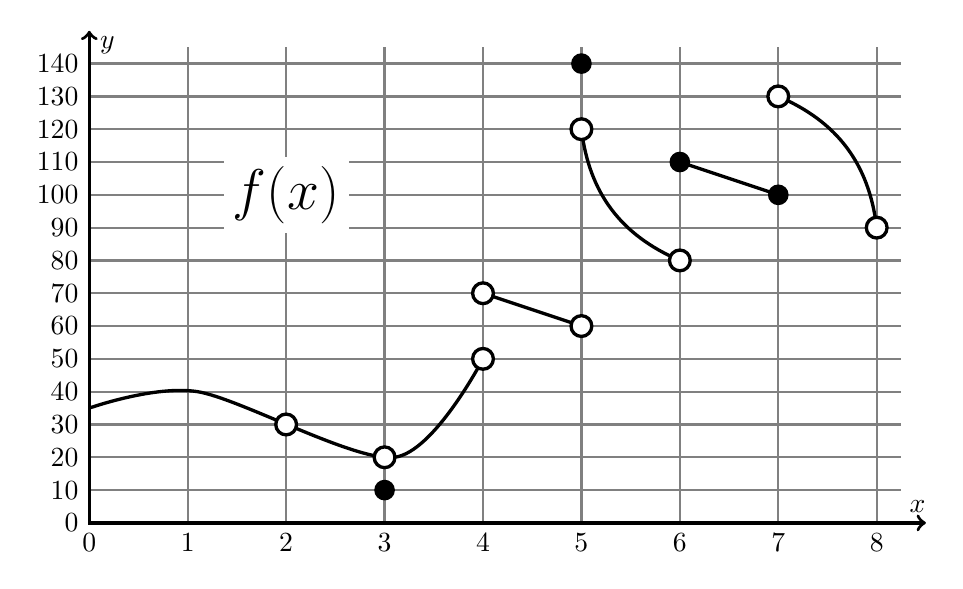
\begin{tikzpicture}
		[scale=1.25, very thick]
	\draw[gray, thick, yscale=1/3] (0,0) grid (8.25,14.5);
	\draw[<->] (0,15/3) -- node[pos=0.03, right] {$y$} (0,0) --  node[pos=0.99, above] {$x$} (8.5,0);
	\foreach \y in {0,10,...,140}
	\draw (0,\y/30) node[left] {\y};
	\foreach \x in {0,...,8}
	\draw (\x,0) node[below] {\x};
	%\draw[rounded corners=10] (0,2/3) -- (1,1) -- (2,2/3) -- (3,1/3) -- (4,5/3);
	\draw[smooth] plot coordinates{(0,3.5/3) (1.1,4/3) (3.1,2/3) (4,5/3)};
	\draw (4,7/3) -- (5,6/3);
	\draw (5,12/3) to [bend right=30] (6,8/3);
	\draw (6,11/3) -- (7,10/3);
	\draw (7,13/3) to [bend left=30]  (8,9/3);
	\foreach \x/\y in {2/3, 3/2, 4/5, 4/7, 5/6, 5/12, 6/8, 7/13, 8/9}
	\draw[black, fill=white] (\x,\y/3) circle (3pt);
	\foreach \x/\y in {3/1, 5/14, 6/11, 7/10}
	\draw[black, fill=black] (\x,\y/3) circle (2.5pt);
	\draw (2,10/3) node[fill,white] {\color{black} \huge$f(x)$};
	\end{tikzpicture}

% VERSION 1 DIAGRAM B (Limits involving infinity)
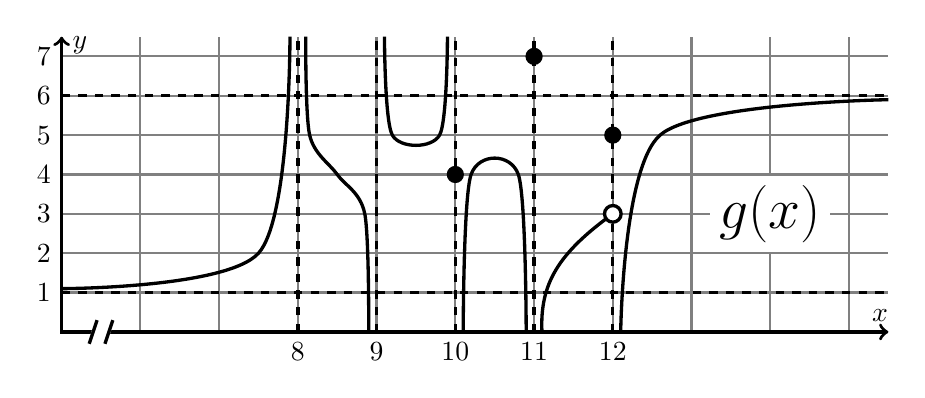
\begin{tikzpicture}
		[very thick,yscale=0.5]
	\draw[gray, thick, yscale=1] (5,0) grid (15.5,7.5);
	\foreach \x in {8,...,12}
	\draw[dashed] (\x,0) -- (\x,7.5);
	\foreach \y in {1,6}
	\draw[dashed] (5,\y) -- (15.5,\y);
	\draw[<->] (5,7.5) -- node[pos=0.03, right] {$y$} (5,0) --  node[pos=0.99, above] {$x$} (15.5,0);
	\foreach \y in {1,...,7}
	\draw (5,\y) node[left] {\y};
	\foreach \x in {8,...,12}
	\draw (\x,0) node[below] {\x};
	\draw[fill, white] (5.45-0.1,-0.3) -- ++(right:0.2) -- ++(0.1,0.6) -- ++(left:0.2) -- ++(-0.1,-0.6);
	\draw (5.45-0.1,-0.3) ++(right:0.2) -- ++(0.1,0.6) ++(left:0.2) -- ++(-0.1,-0.6);
%	\draw[rounded corners=20] (5,1) -- (6,1) -- (6,7.5);
	\draw[smooth] plot coordinates {(5,1.1) (7.5,2) (7.9,7.5)};
	\draw[smooth] plot coordinates {(8.1,7.5) (8.15,5) (8.5,4) (8.85,3) (8.9,0)};
	\draw[smooth] plot coordinates {(9.1,7.5) (9.2,5) (9.8,5) (9.9,7.5)};
	\draw[smooth] plot coordinates {(10.1,0) (10.2,4) (10.8,4) (10.9,0)};
	\draw (11.1,0) to [bend left=18] (12,3);
	\draw[smooth] plot coordinates {(12.1,0) (12.6,5) (15.5,5.9)};
	\foreach \x/\y in {12/3}
	\draw[black, fill=white,yscale=2] (\x,\y/2) circle (3pt);
	\foreach \x/\y in {12/5, 11/7, 10/4}
	\draw[black, fill=black,yscale=2] (\x,\y/2) circle (2.5pt);
	\draw (14,3) node[fill,white] {\color{black} \huge$g(x)$};
	\end{tikzpicture}